% !TEX root = ../../fyp.tex
\documentclass[../../fyp.tex]{subfiles}

\begin{document}
We carry out all experiments using GloVe word embeddings \cite{pennington} since all of the studies reproduced use some version of these and because these embeddings performed optimally in both \cite{moore2018} and \cite{bhuwandhingra2017} when dealing with NN based approaches. Since these word embeddings are case insensitive, we lowercase all tokens and carry out tokenization using the Spacy library with the default token filter (\S\ref{sec:filtering_embeddings}) to remove all emails and URLs from the text.

When determining parameters for each model, the following order is adopted; first, parameters from the original paper are set, while also referring to any accompanying source code which could include parameters missing from the papers. Where unavailable, we use configurations adopted by third-party implementations based on their reported results. Finally, we set any other parameters intuitively, based on the respective setting from models with similar architectures. 

As we shall outline, a non-trivial portion of the studies covered omitted essential parameter settings, such as the learning-rate of a model or the number of hidden units used, which drastically hinder their reproducibility. These omissions would be understandable provided the work is supplemented with source-code, however, this was also unobtainable or excluded in most cases.

Parameters such as the batch-size and duration of training are assumed based on online implementations, which report results similar to the original work. To account for this,following \cite{moore2018}, we adopt early-stopping with a patience of 10 epochs, a maximum allowance of 300 epochs and a minimum of 30 epochs, monitoring the loss metric of each model at every epoch. 

We first provide a brief overview of each approach, which is followed by a description of the challenges faced in reproducing each approach in particular, and the counter-measures taken. Finally, we contrast the results obtained from our experiments with those reported in the original work. Since he effect of the random seed on parameter initialization is statistically significant \cite{reimers2017} as cited in \cite{moore2018}, we report mean values from 3 separate runs using different random seed values, for each experiment. 

\subsection{TD-LSTM}
The work carried out by Tang et al 2016 was one of the first to employ LSTM based methods for the task of TSA. Three variants were developed for their experiments, first, a baseline LSTM model which did not take any target information into account. A Target Dependent(TD) LSTM integrated target information by concatenating the target vector to both left and right contexts, and using two separate LSTMs for each. Finally, a Target-Connected(TC) LSTM also adopted two LSTMs, however the target vector information was concatenated to each word in the context, rather than the context as a whole as in the TD-LSTM. This modification incurs a cost on computation time, as it effectively doubles the embedding dimension of each word. Each variant is followed by a softmax layer which is used to obtain the final classification of the sentence.  

The authors use the Dong et al. 2014 dataset, and experiment with both 100-dimension and 200-dimension twitter based GloVe embeddings. Furthermore, LSTM weights are initialized using U(-0.003,0.003) and training is carried out using stochastic gradient descent with a lerning rate of 0.01.

A notable omission in Tang et al. 2016 as well as the reproduction carried out by Moore  et al. 2018 is the hidden unit count for each LSTM cell. 

To choose a value for this parameter, experiments were carried out for each LSTM variant with 200 and 300 hidden units and both were found to converge on similar results. Since the latter requires more computational resources in training we assume a value of 200 for the results presented herein. 

The insignificant downstream differences between these two variants notwithstanding, the omission of this parameter makes reproduction attemps more challenging, and leaves room for uncertainty when comparing results to the original work. 

Finally, similar to Moore et al 2018, we ignore the reported 'softmax clipping threshold' of 200 as the implications of this remained misunderstood, and no further elaboration on the parameter is provided by Tang et al. 2016. 

As there was no mention of the batch-size or the amount of hidden units used in the kernel of the LSTMs these were set to be 200 and 64 respectively. These values were taken from online public implementations which quoted results similar to those reported in [Tang2016a]

Following on the approach by Moore, we vary the embeddings being used in termed of dimensionality so as to test the observed improvement in results with its increase. 

We also increase the upper bound to 300d by including the two variants of the glove embeddings which are sourced from a wider vocabulary, not exclusive to twitter, which could make them better suited for the restaurants and laptops datasets. 

Finally, the larger of these two variants also takes into account another aspect by differentiating between uppercase and lowercase letters in tokens. 

\begin{figure}[!ht]
	\centering
	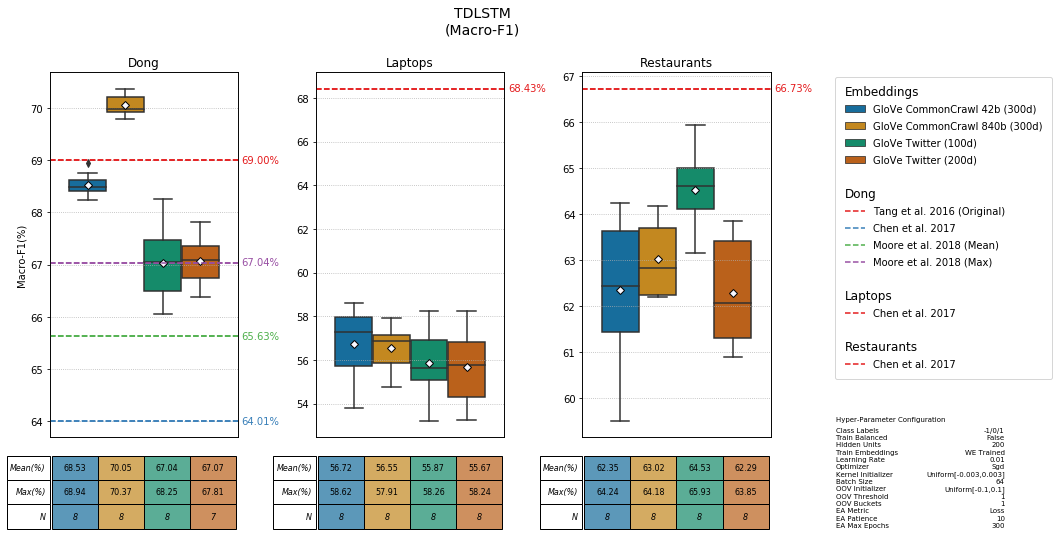
\includegraphics[width=\textwidth]{tdlstm_orig_macrof1.png}
	\caption{TD-LSTM Macro-F1 Results, $N$ refers to the number of runs carried out.}
	\label{fig:ffnn}
\end{figure}

We consider the performance of the TD-LSTM as it is the most commonly quoted variant compared in the literature. 

Comparing macro-f1 scores to account for the class imbalances in each dataset we note that the 300d GloVe variants outperform the 100d and 200d embeddings, even though the latter are not sourced from twitter as is the dataset. The 840b variant obtains the best score, suggesting that there is valuable information contained in the case-sensitivity of tokens.


When considering the laptops and restaurants dataset, which differ to dong in terms of class balance and sample length [REF Chapter on datasets], performance drops significantly. 

Although the non-twitter embedding variants slightly outperform their counterparts in the laptop dataset, the best mean result is 56.55\% indicating the model's poor capacity for learing from the dataset. 

The same can be said for the restaurants dataset, considering the wide variance in the results observed using any embedding with the best results being counterintuitively obtained by the 100d twitter-sourced glove variant.

When considering the results obtained for the Dong dataset, we note that both 100d and 200d glove embeddings perform similarly, with a slight edge in the mean of the 200d variant. This notwithstanding, both variants' performance is markedly less than that reported in the original paper [Tang], which as stated in [Moore], can be attributed reporting only results from singular runs, thus not taking into account the downstream effects of differences in random initializations of weights. 

Finally, the performance of the 300d embedding variants in comparison, is in accordance with the upward trend with increased dimensionality noted in [Moore]

When comparing the results obtained in the laptops and restaurants dataset to those reported in [Chen2017] there is a significant difference irrespective of the embedding used. Although this can also be caused by randomness in the wegiht initializations (no mention of multiple runs is made), it is interesting to note that the opposite phenomena is observed when considering the dong dataset. In this instance the result reported by [Chen2017] is substantially lower than the rest.

This discrepency may be the result of the different approaches that were adopted to account for unknown parameters in the original work [Tang2016a] which were similarly left unreported in [Chen2017].

\subsection{IAN}

The Interactive Attention Network (IAN) model [Dehong Ma et. al 2017] separates the input sentence into target and context and feeds the vector representation of these elements to two separate LSTM units. The authors subsequently use max-pooling on the hidden states of these LSTM units and employ an attention mechanism to attend on the output of each LSTM unit with respect to the other's max-pooled hidden state vector. This produces a vector representation of the context weighted by the attention scores with respect to the target and vice-versa. These representations are then concatenated and fed to a softmax classifier which produces a probability distribution over the class labels, the highest of which is taken to be the final predicted class. 

A defining characteristic of this approach is the fact that it is not solely the context's represenation which is dependent on the target, but the target representation itself is affected by its context. 

\begin{figure}[!ht]
	\centering
	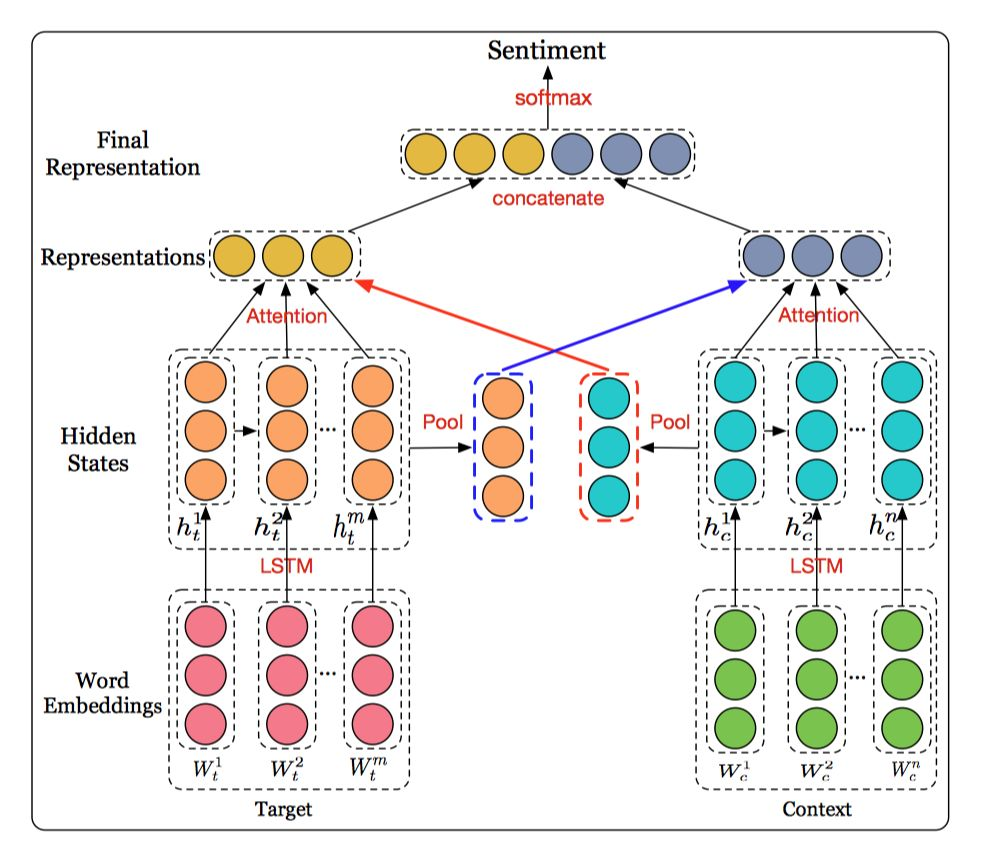
\includegraphics[width=\textwidth]{ian_arch.jpeg}
	\caption{Architecture of the IAN Model [Dehong Ma et al. 2017]}
	\label{fig:ffnn}
\end{figure}

The authors make use of a momentum optimizer [Qian et al. 1999] when training their model, however they do not mention the specific momentum parameter that is used when obtaining the reported results. The authors also omit the learning rate hyper-parameter and the batch-size used in their training, both of which are correlated to the momentum hyper-parameter previously mentioned which further exacerbates the problem. 

Finally, the authors remark that GloVe [Pennington et al. 2014] embeddings are used with a dimentionality matching that of the hidden unit count in each of the LSTM units, namely 300. It must be noted however that there are two variants of these embeddings with that dimentionality, with substantially different source-vocabulary sizes and only one of which is case-sensitive.

We use values reported in a more recent paper [Zhang et al. 2018] for the momentum, learning-rate and batch size parameters for the default configuration of this model since these parameters are intertwined and in their work [Zhang et al. 2018] report promising results. 

We further consider this 'default configuration' as a baseline for the model and evaluate its performance on the datasets reported in the original work as well as the Dong twitter dataset. Furhtermore, we also include four different variants of the GloVe embeddings, 100 and 200 dimentionality twitter variants and both of the aforementioend 300 dimentionality variants so as to observe the difference in downstream performance these make with respect to the reported results. 

\begin{figure}[!ht]
	\centering
	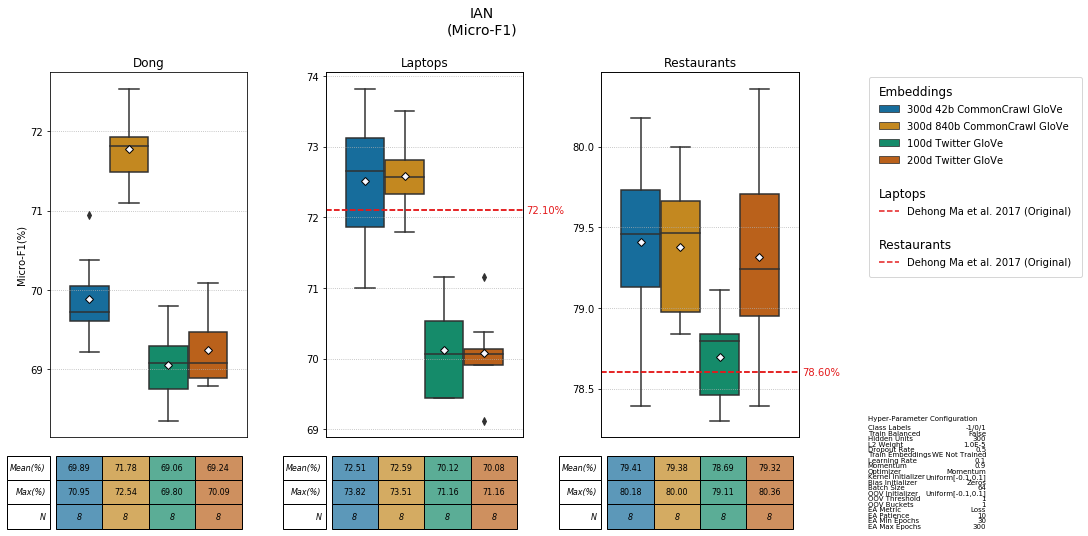
\includegraphics[width=\textwidth]{ian_default_microf1.png}
	\caption{IAN Micro-F1 results (compared with originally reported results)}
	\label{fig:ffnn}
\end{figure}

\begin{figure}[!ht]
	\centering
	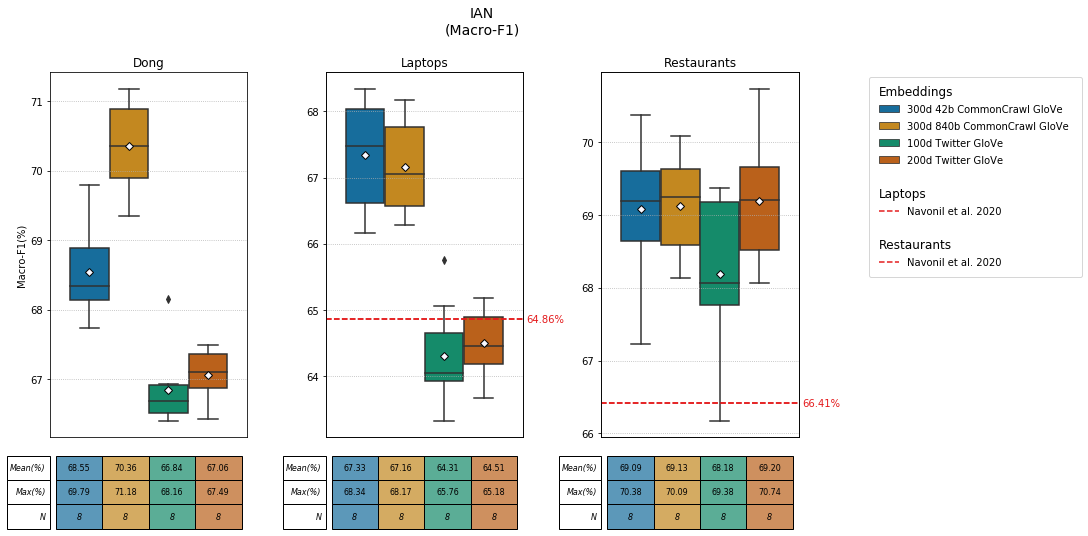
\includegraphics[width=\textwidth]{ian_default_macrof1.png}
	\caption{IAN Macro-F1 results (compared with results reported in [Navonil et al. 2020])}
	\label{fig:ffnn}
\end{figure}

We first compare the micro-F1 (accuracy) results obtained in the our experiments with those reported in the original work [Ma et al. 2017] for the laptops and the restaurants dataset as these are the only metrics which were cited. It is worth pointing out once more that both of these datasets are heavily skewed in their class distribution [REF: datasets chapter for more info] which confines the validity of this metric.

This notwithstanding, in both datasets when employing both variants of the 300d GloVe embeddings we find that the reported micro-f1 results are considered conservative when compared to the mean value of the same metric in our experiments. 

The authors do not mention the number of runs that were performed or whether multiple runs were performed, which may explain this discrepancy. We can observe that both reported metrics fall within the range of results obtained with the 42b 300d GloVe embedding, which may suggest that this was the variant the authors were referreing to in their work. 

Recently, a novel approach was presented in [Novanil et al. 2020] which included the IAN architecture as a baseline and report macro-f1 scores for the skewed datasets. In their work, the authors report a learning rate of 0.002 as opposed to 0.1 which was employed in our work. 

We observe similar, if not more pronounced, differences when considering the 300d GloVe variants in both laptop and restaurants datasets, with the reported metrics in both cases falling squarely below the range of values we obtain in our experiments. 

Although this discrepenacy in both cases can be considered 'favorable', it nonetheless continues to underscore the importance of providing all parameter settings for these models to facilitate reproduction by mitigating the overhead involved in attempting to recreate the original results. 

Moreover, the importance of reporting metrics which take into account dataset characteristics as outlined in [REF: chapter on metrics] and which take into account the downstream effects of randomness in the initialization process [Gurevych, Moore] continues to emerge from these results. 

\subsection{LCR-ROT}
From the approaches described thus far, we observe that utilizing attention mechanisms to affect the representation of a context concerning its target is effective when tackling TSA tasks. This may be considered fairly intuitive, however, as we have seen \cite{dehongma2017} present a compelling argument with their IAN model that the inverse, in favor of using attention mechanisms to affect the target representation concerning its context as well. \cite{zheng2018} expand upon this idea in their work presenting a Left-Center-Right Rotary Attention network (LCR-ROT) in several ways, albeit at the cost of a heavier computational load. 

First, similar to other works such as \cite{tang2016} and \cite{chen2017}, the authors consider the left and right contexts of a target separately as opposed to a single context vector which makes the model more robust when considering the same sentence for different targets. 

Secondly, the authors employ Bi-directional LSTMs, which enable the model to extract sequential feature data in both directions of a sequence. This comes at the cost of double the parameters that the model must learn since it is achieved by stacking the hidden states of two separate LSTMs processing the sequence in opposite directions. Three BiLSTMs are used for the left and right contexts and the target respectively. 

An initial, \textit{Target2Context}, attention model is used to weight both left and right context representations against a target representation obtained through average-pooling, producing target-aware context representations. The rotary attention mechanism characterizes the inverse of this process, using both target-aware context representations in combination with a second \textit{Context2Target} attention model to construct two separate left-aware and right-aware target representations. 

Finally, all four components are used in conjunction as the sentence feature vector which is fed to a softmax classifier to obtain the sentiment classification. 
\begin{figure}[!ht]
	\centering
	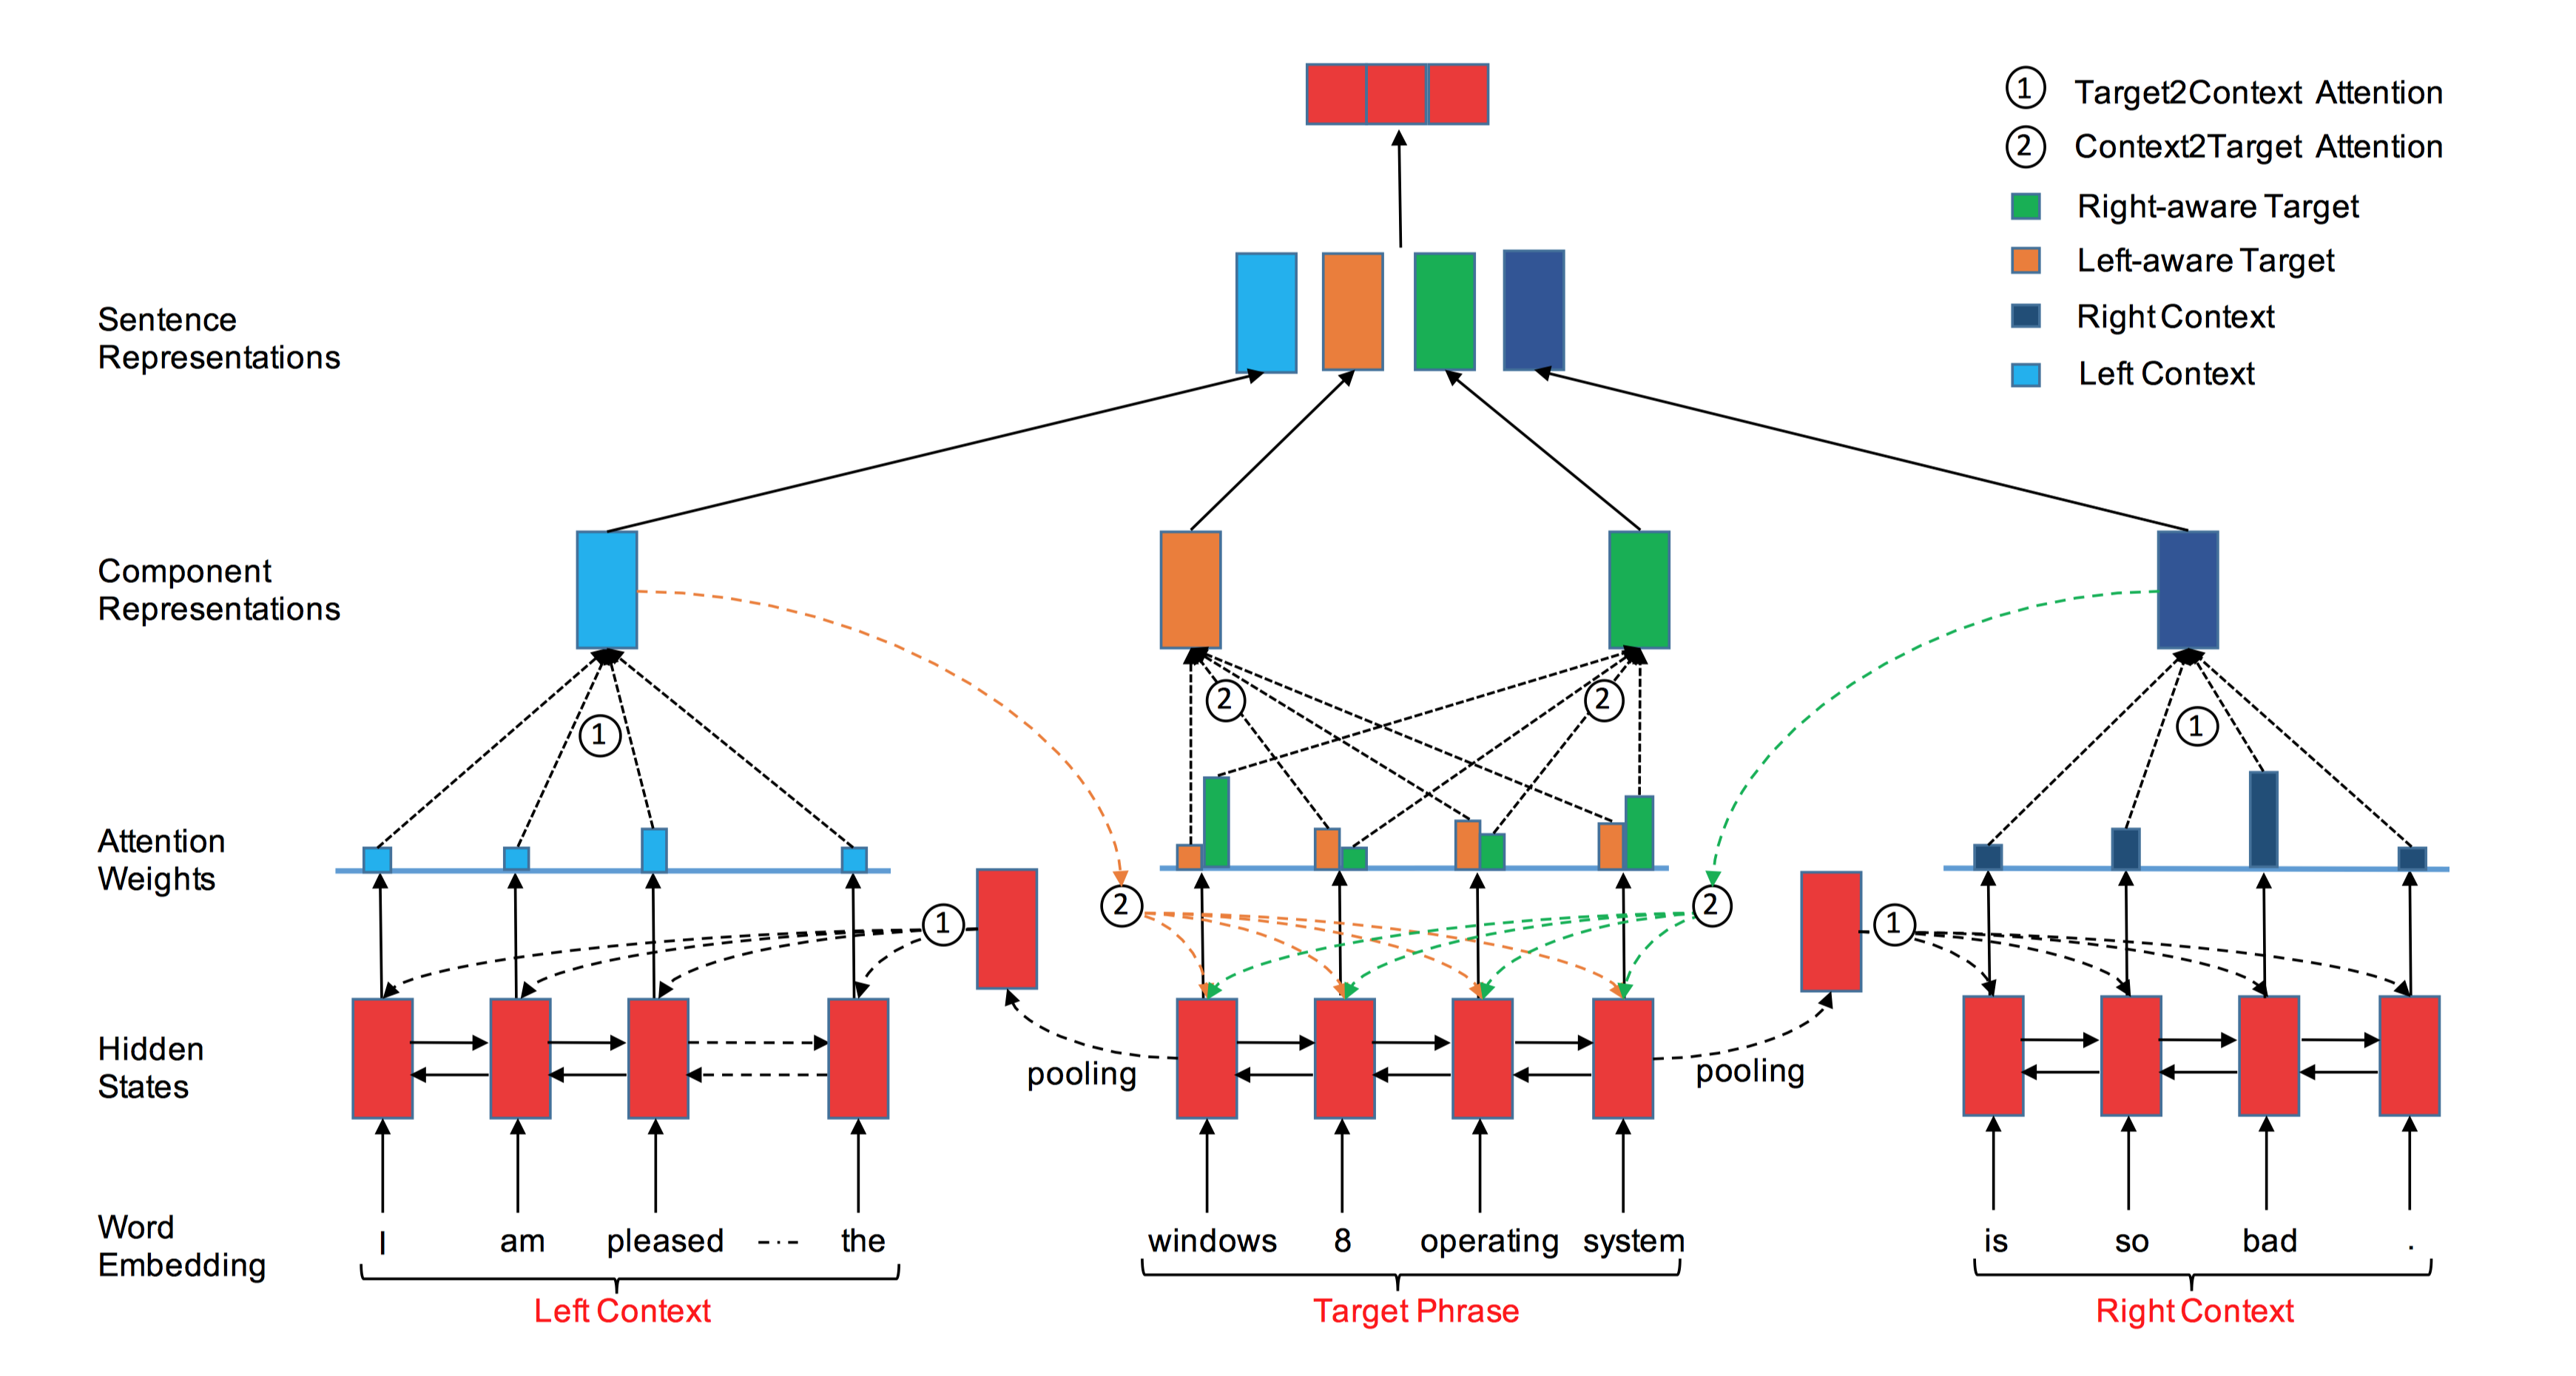
\includegraphics[width=\textwidth]{lcrrot_architecture.png}
	\caption{Left-Center-Right Separated Neural Network Architecture \cite{zheng2018} illustrating the construction of each constituent component of the final sentence representation. Bi-LSTMs are employed for the initial feature extraction followed by two attention models, \textit{Target2Context} and \textit{Context2Target}, which produce target-aware context representations as well as left and right context-aware target representations.}
	\label{fig:ffnn}
\end{figure}

When attempting to reproduce the approach as described in \cite{zheng2018}, we note that this work provides the best coverage of important parameters thus far. The authors further indicate their intention to make the source code of their model publically accessible. Although the paper provides no direct link, the repository was sufficiently easy to locate manually. The repository contains an example, which specifies values for the remaining, otherwise unspecified parameters. In this case, these are the batch-size and training duration. Although unclear whether meant merely as a suggestion, we use this configuration for our reproduction experiments on the assumption that this configuration would be the most well-educated even in this eventuality.   

However, a more pressing concern is the lack of specificity when describing the word embeddings used for their experiments. We have previously outlined the differences in the two variants of 300-dimension GloVe embeddings, and have repeatedly produced varying results in each of our tests. \cite{zheng2018} cite \cite{wang2018} and \cite{tang2016} as motivation for their choice of embeddings; however, these approaches report using different variants to one another.

Furthermore, the authors do not specify whether embeddings were trained further in their experiments. When referring to the codebase, we note both approaches, with the code for further embedding training being disabled. We assume this to imply that excluding embeddings from the training process provided superior results and adopt the same approach in our experiments. 

Finally, we draw attention to the use of accuracy (macro-f1) as the definitive metric for performance, particularly when considering the laptops and restaurants datasets. As previously mentioned, the composition of these datasets' constituent classes is heavily skewed. We have described how easily accuracy falls victim to overly-optimistic and biased results by not accounting for this imbalance.   

\begin{figure}[!ht]
	\centering
	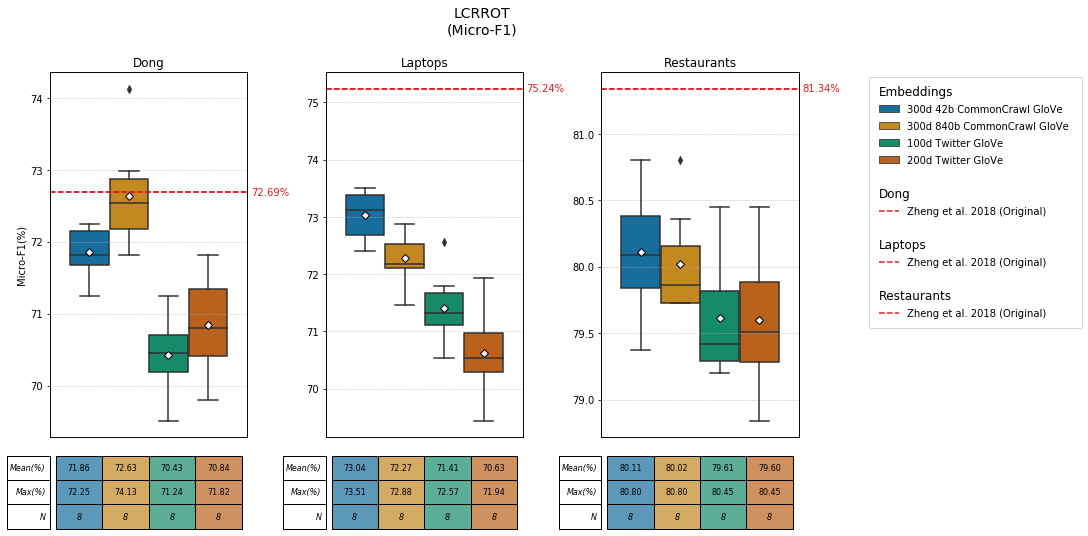
\includegraphics[width=\textwidth]{lcrrot_default_microf1.png}
	\caption{LCR-ROT Micro-F1 results (compared with originally reported results)}
	\label{fig:ffnn}
\end{figure}

\begin{figure}[!ht]
	\centering
	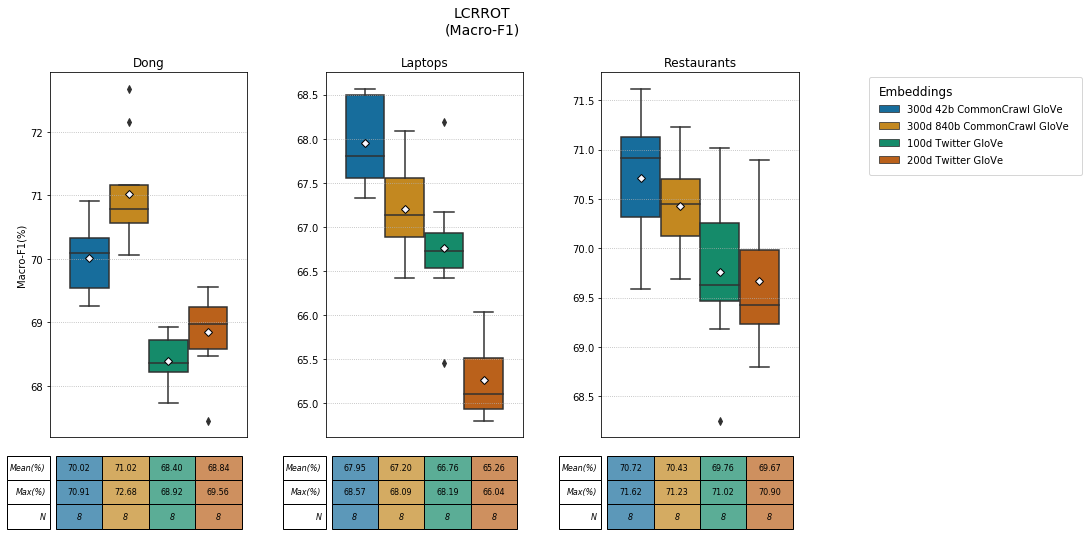
\includegraphics[width=\textwidth]{lcrrot_default_macrof1.png}
	\caption{LCR-ROT Macro-F1 results}
	\label{fig:ffnn}
\end{figure}

Similar to the previously mentioned studies, we assume the reported metrics are optimal, as the authors did not mention multiple runs. When considering the Dong dataset, our results suggest that the authors employed the larger 840b variant of the GloVe embeddings. The reported micro-f1, in this case, falls within the mean (-0.06), as opposed to the 42b variant, which performs markedly worse. 

We note that the principles adopted in the LCR-ROT approach's more sophisticated modeling of context and target relations are substantiated. The model outperforms the previous works across all experiment configurations we investigate. Despite this, we were unable to reproduce the reported micro-f1 metrics for the Laptops and Restaurants datasets. The more substantial discrepancy between results for these two datasets, when compared to the Dong dataset, is likely a consequence of the latter's less pronounced class imbalance. [REF to datasets chapter] 

We observe another evident by-product of this distinction in the magnitude of deviation in macro-f1 scores and micro-f1 scores. Considering the best-performing mean scores for each dataset, the macro-f1 scores for the Dong dataset deviates from its respective micro-f1 counterpart by 1.61 points. Comparatively, this figure increases to 5.09 and 9.38 for the Laptops and Restaurants datasets' best-performing configurations. This difference is replicated across all embedding configurations and is an indication of the degree to which the micro-f1 metric falls short in these circumstances.

Finally, we note that in all previously presented experiments, the 840b GloVe embedding consistently outperforms its 42b counterpart in the Dong dataset. The nature of the Dong dataset, being sourced from a social media platform that encourages a relaxed demeanor and enforces brevity, leading to samples that typically ignore correct grammar and punctuation. Initially, it may seem counter-intuitive that the case-sensitive embeddings would perform better in this domain. However, we surmise that by often ignoring the case, in the rare instances which adhere to it, such as proper nouns, provide more information than in other, more formal and verbose, datasets. 

\subsection{Concluding Remarks}
We have documented herein the process of reproducing three critical studies employing increasingly complex structures to further the field of TSA. In doing so, we have elucidated the following challenges and suggestions to mitigate them accordingly: 

\begin{itemize}
	\item We have outlined the detrimental effects that lack of specificity has on this process, consuming more time and resources, thereby setting back further development. While ensuring that all pertinent parameter values original reports provide all pertinent parameters is ideal, the optimal solution is to strive to make the accompanying code publically available. 
	\item We have illustrated in each case how reporting singular, optimal scores is insufficient, given the variance observed in each of our experiments when carrying out multiple runs with different random seeds. Although limited in our work by resources, we acknowledge that this approach may carry increasing insight into a model with an even higher number of runs. 
	\item Finally, we have shown that careful attention is imperative when considering the performance metric to report, for the datasets used. Notably, it is evident that macro-f1 scores are more robust in this field and give a more precise, albeit less optimistic, measure of a model's performance.
\end{itemize}


\end{document}